\documentclass[../TDE7_ocrsf.tex]{subfiles}%

\begin{document}
% TODO: Refaire figure et axe pour déphasage : problème unité.

\section[s]"2"{Modélisation d'un haut-parleur}
\enonce{%
	\begin{minipage}{0.55\linewidth}
		On modélise la partie mécanique d'un haut-parleur comme une masse $m$, se
		déplaçant horizontalement le long d'un axe $(Ox)$. Cette masse est reliée
		à un ressort de longueur à vide $\ell_0$ et de raideur $k$ et subit une
		force de frottement fluide~: $\vec{f} = -\alpha \vec{v}$. Elle est par
		ailleurs soumise à une force $\vec{F}(t)$, imposée par le courant $i(t)$
		entrant dans le haut-parleur, qui vaut~: $\vec{F}(t) = K i(t) \vec{u}_x$
		où $K$ est une constante. On travaille dans le référentiel du laboratoire
		$(O, \vec{u}_x , \vec{u}_y)$. On suppose que le courant est de la forme
		$i(t) = I_m \cos(\wt)$.
	\end{minipage}
	\hfill
	\begin{minipage}{0.45\linewidth}
		\begin{center}
			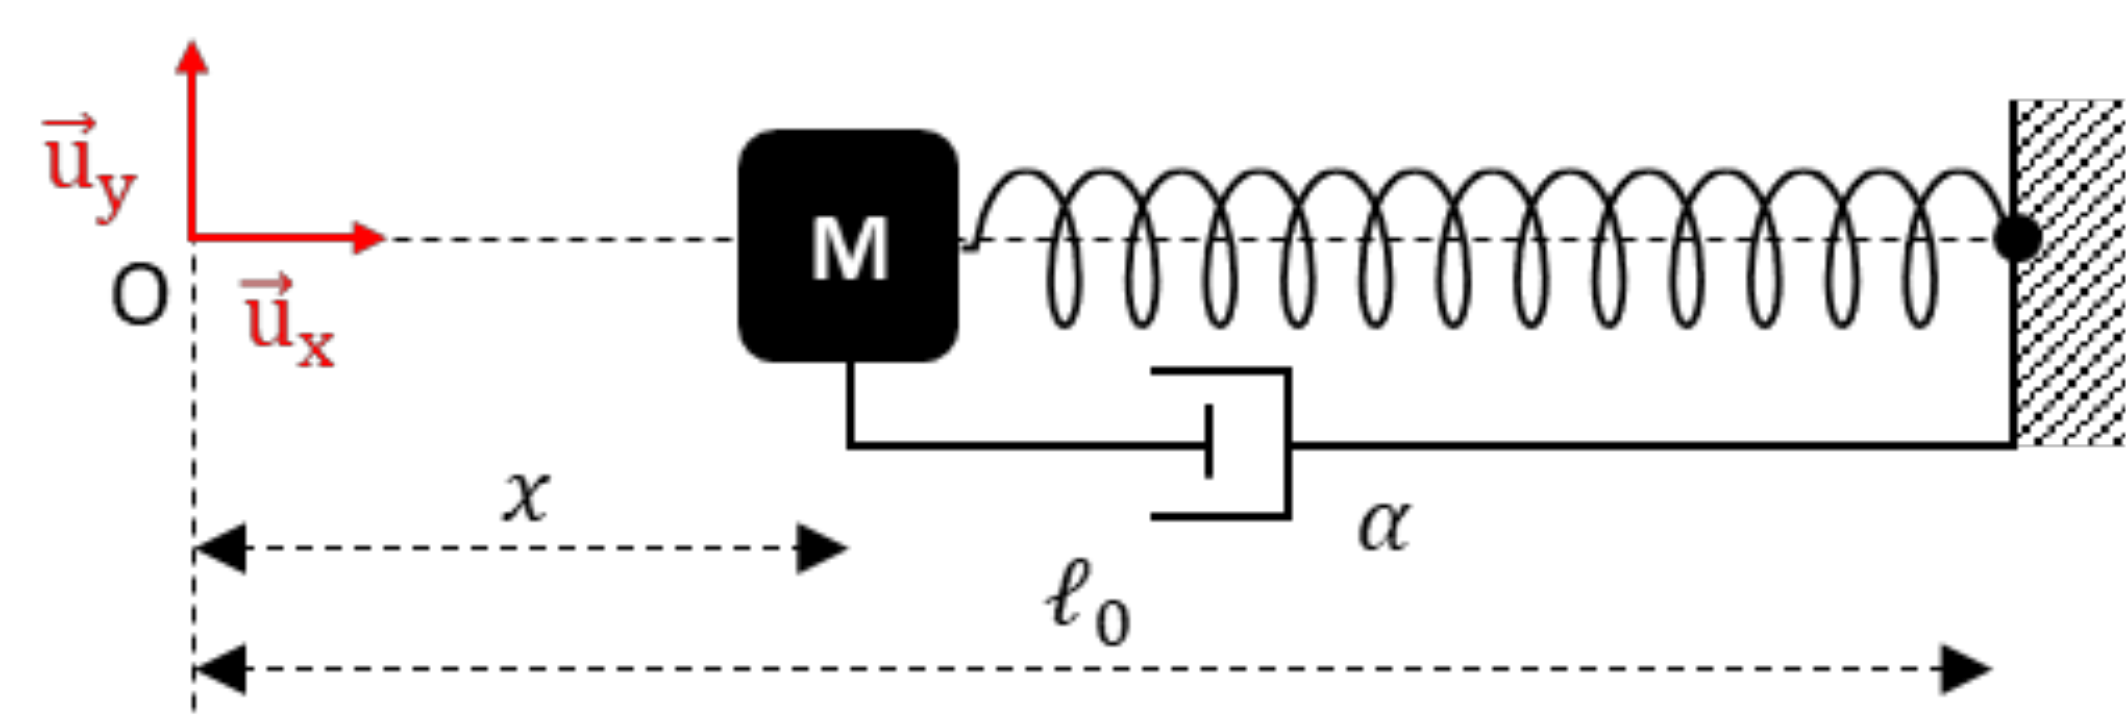
\includegraphics[width=.9\linewidth]{hp_1}
		\end{center}
	\end{minipage}

	\begin{tcb}(data)<lfnt>{Données}
		$m = \SI{10}{g}$, $K = \SI{200}{N.A^{-1}}$ et $I_m = \SI{1.0}{A}$.
	\end{tcb}
}

\QR{%
	Écrire l'équation différentielle vérifiée par $x(t)$, la position de
	la masse $m$.
}{%
	~
	\smallbreak
	\vspace{-18pt}
	\begin{minipage}{0.43\linewidth}
		\begin{itemize}
			\item[b]{Système} : masse~;
			\item[b]{Référentiel} : $\Rc_{\rm sol} (O,x,y,t)$~;
			\item[b]{Position de la masse} : $\OM = x\ux$~;
			\item[b]{Longueur ressort} : $\vv{MA} = \ell\ux$~;
			\item[b]{Longueur à vide} : $\vv{OA} = \ell_0\ux$~;
			\item[b]{Longueur relative} :\\
			      $(\ell - \ell_0)\ux = \vv{MO} = -x\ux$.
		\end{itemize}
	\end{minipage}
	\hfill
	\begin{minipage}{0.57\linewidth}
		\textbf{Bilan des forces}~:
		\begin{enumerate}
			\item Poids $\Pf = -mg\uy$~;
			\item Réaction du support $\vv{R} = R\uy$~;
			\item Force de rappel du ressort\\
			      $\vv*{F}{\rm ressort} = k(\ell - \ell_0)\ux =
				      k\vv{MO} = -kx\ux$~;
			\item Force de frottement fluide $\vv{f} = -\alpha\vf =
				      -\alpha\dot{x}\ux$~;
			\item \textbf{Force excitatrice} $\Ff = KI_m\cos(\wt)\ux$.
		\end{enumerate}
	\end{minipage}

	\begin{gather*}
		\beforetext{Avec le PFD~:}
		m\af = \Pf + \vv{R} + \Ff_{\rm ressort} + \vv{f} +\Ff\\
		\Leftrightarrow m\left(
		\begin{array}{c}
				\DS\dv[2]{x}{t} \\
				0
			\end{array}
		\right)
		=
		\left(
		\begin{array}{c}
				-kx -\alpha v + KI_m\cos(\wt) \\
				-mg + R
			\end{array}
		\right)
	\end{gather*}
	La projection sur $\uy$ montre que la réaction du support compense le poids.
	Sur l'axe $\ux$ on trouve
	\begin{gather*}
		\boxed{m \dv[2]{x}{t} + \alpha \dv{x}{t} + kx = KI_m\cos(\wt)}
	\end{gather*}
}

\QR{%
	La mettre sous forme canonique et identifier les expressions de la
	pulsation propre $\w_0$ et du facteur de qualité $Q$.
}{%
	Sous forme canonique, cela devient
	\begin{gather*}
		\Leftrightarrow
		\boxed{\ddot{x} + \frac{\w_0}{Q}\dot{x} + \w_0{}^2x =
			\frac{KI_m}{m}\cos(\wt)}\\
		\qavec
		\boxed{\w_0 = \sqrt{\frac{k}{m}}}
		\qet
		\boxed{Q = \frac{\sqrt{km}}{\alpha}}
	\end{gather*}
}

\QR{%
	Justifier qu'en régime permanent: $x(t) = X_m \cos(\wt + \phi)$
}{%
	On sait que pour une entrée sinusoïdale, un système aura une solution
	homogène donnant un régime transitoire et une solution particulière de
	la forme de l'entrée~: en RSF, on étudie le régime permanent où seule la
	solution particulière est conservée, et on pourra donc écrire $x(t) =
		X_m\cos(\wt+\F)$.
}

\QR{%
On pose $\xul{x}(t) = \xul{X}e^{\jwt}$. Déterminer
l'expression de l'amplitude complexe $\xul{X}$.
}{%

En passant en complexes,
\begin{gather*}
	(\jw)^2\Xu + \jw\frac{\w_0}{Q}\Xu + \w_0{}^2\Xu = \frac{KI_m}{m}\\
	\Leftrightarrow
	\xul{X} =
	\frac{KI_m}{m}\times
	\frac{1}{\w_0{}^2 - \w^2 + \dfrac{\jj}{Q}\w\w_0}
	\Leftrightarrow
	\boxed{
		\xul{X} = \frac{KI_m}{m\w_0{}^2}\frac{1}{1 -
			\left( \dfrac{\w}{\w_0} \right)^2 +
			\jj\dfrac{\w}{Q\w_0}}
	}
\end{gather*}
}

\QR{%
	Exprimer $X_m(\w)$. Existe-t-il toujours une résonance?
}{%
	En réels, on trouve
	\begin{gather*}
		\boxed{
			X(\w)
			= \abs{\xul{X}}
			= \frac{KI_m}{m\w_0{}^2}\frac{1}{
				\sqrt{\left( 1 - \left(\dfrac{\w}{\w_0}\right)^2 \right)^2
					+ \left(\dfrac{\w}{Q\w_0}\right)^2}}
		}
	\end{gather*}
	Elle est maximale quand le dénominateur est minimal. Après calcul,
	on trouve
	\begin{itemize}[leftmargin=60pt]
		\item{}[$\mathbf{Q \leq 1/\sqrt{2}}$] : l'amplitude est maximale pour
		      \[\boxed{\w = 0 \qet X(0) = \frac{KI_m}{m\w_0{}^2}}\]
		\item{}[$\mathbf{Q > 1/\sqrt{2}}$] : l'amplitude est maximale pour
		      \[\boxed{\w_r = \w_0 \sqrt{1 - \frac{1}{2Q^2}} < \w_0}
			      \qet
			      \boxed{X(\w_r) = \frac{KI_m}{m\w_0{}^2}
				      \frac{Q}{\sqrt{1 - \frac{1}{4Q^2}}}}
		      \]
	\end{itemize}
	De ce résultat, nous observons qu'il \textbf{n'y a pas toujours
		résonance en élongation}, et que \textbf{la résonance est d'autant
		aiguë que $\mathbf{Q}$ est élevé}.
}

\enonce{%
	On a tracé ci-dessous les courbes de $X_m (\w)$ et de
	$\phi(\w)$.
	\begin{center}
		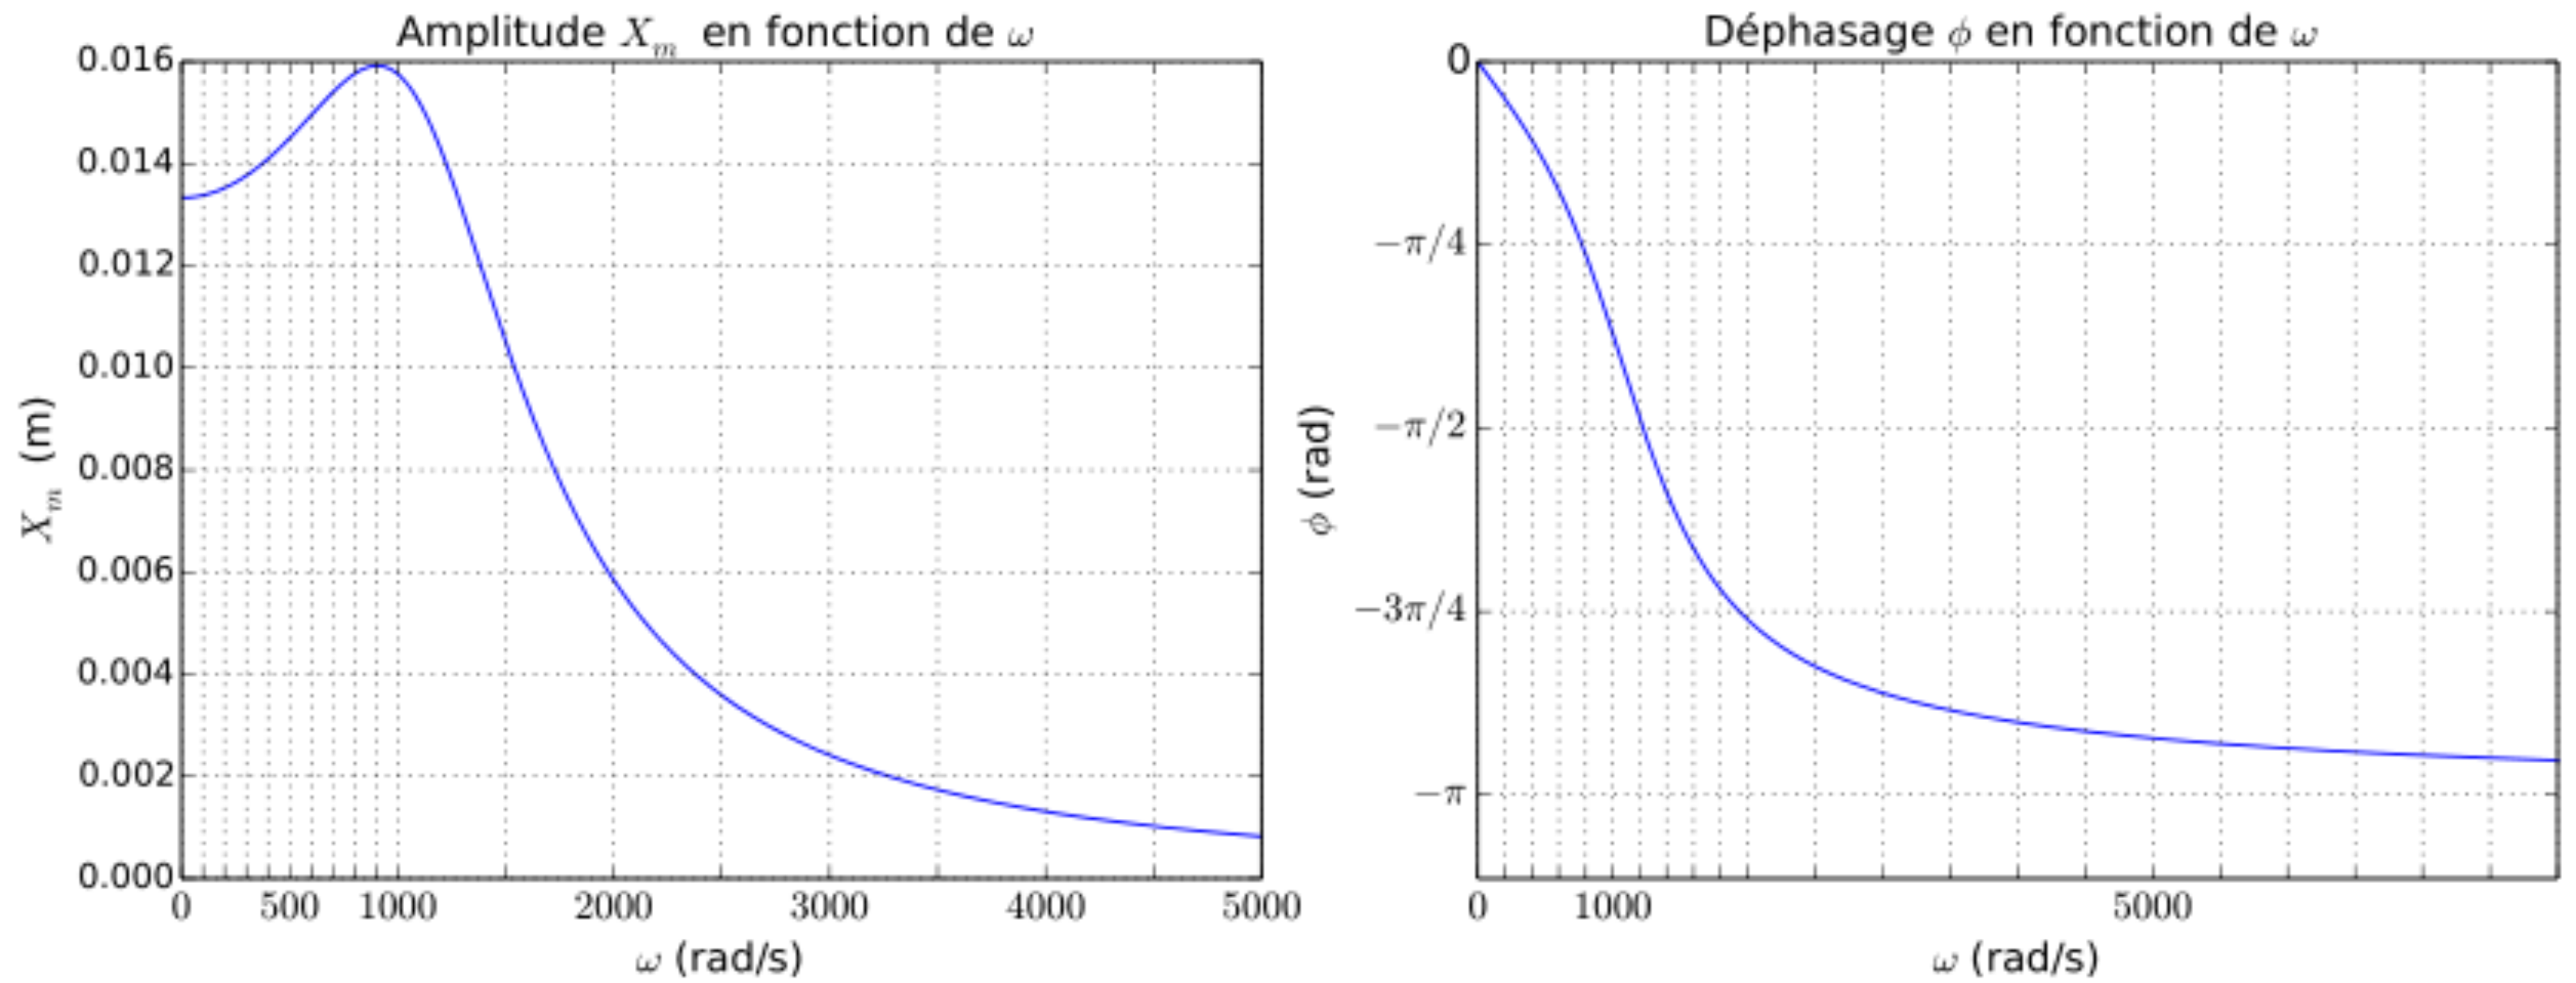
\includegraphics[width=.8\linewidth]{hp_2}
	\end{center}
}

\QR{%
	Pour quelle pulsation le déplacement est-il en quadrature de phase
	avec la force excitatrice~? Déterminer alors graphiquement la pulsation
	propre $\w_0$.
}{%
	Le déplacement est en quadrature de phase si la différence de phase
	est de $\pm\pi/2$. Sur le graphique de droite, on le trouve à $\w =
		\SI{1100}{rad.s^{-1}}$. Or, c'est à $\w = \w_0$ qu'on trouve une
	quadrature de phase, puisqu'alors $\Xu$ est un imaginaire pur. Ainsi,
	\[\w_0 = \SI{1100}{rad.s^{-1}}\]
	On pourrait déterminer le facteur de qualité en trouvant que le maximum
	d'amplitude se trouve à $\w_r = \SI{900}{rad.s^{-1}}$.
}
\end{document}
